% gen_event Usage Guide
% A complete introduction to gen_event with architecture diagrams and examples.
% Compile with: xelatex gen_event_architecture.tex (run twice for TOC)
\documentclass[a4paper,11pt]{article}

% ============================================================
% Packages
% ============================================================
\usepackage{fontspec}
\usepackage{xeCJK}
\setCJKmainfont[BoldFont=STHeiti, ItalicFont=STKaiti]{STSong}
\setCJKsansfont{STHeiti}
\setCJKmonofont{STFangsong}

\usepackage[margin=2.5cm]{geometry}
\usepackage{graphicx}
\usepackage{xcolor}
\usepackage{hyperref}
\usepackage{listings}
\usepackage{booktabs}
\usepackage{longtable}
\usepackage{enumitem}
\usepackage{tikz}
\usepackage{tcolorbox}
\usepackage{fancyhdr}
\usepackage{titlesec}
\usepackage{amsmath}
\usepackage{amssymb}
\usepackage{float}
\usepackage{pifont}

\usetikzlibrary{arrows.meta, positioning, shapes.geometric, fit, calc, backgrounds, decorations.pathreplacing}

\tcbuselibrary{listings, skins, breakable}

% ============================================================
% Color Definitions
% ============================================================
\definecolor{erlred}{HTML}{A4070A}
\definecolor{erlblue}{HTML}{2B5EA7}
\definecolor{erlgreen}{HTML}{2E7D32}
\definecolor{erlyellow}{HTML}{F9A825}
\definecolor{erlpurple}{HTML}{6A1B9A}
\definecolor{erlmodule}{HTML}{D84315}
\definecolor{erlinit}{HTML}{00897B}
\definecolor{erlpid}{HTML}{E65100}
\definecolor{erlname}{HTML}{6A1B9A}
\definecolor{codebg}{HTML}{F5F5F5}
\definecolor{codeborder}{HTML}{CCCCCC}
\definecolor{tipbg}{HTML}{E8F5E9}
\definecolor{warnbg}{HTML}{FFF3E0}
\definecolor{notebg}{HTML}{E3F2FD}
\definecolor{darkgray}{HTML}{333333}

% ============================================================
% Hyperref Setup
% ============================================================
\hypersetup{
    colorlinks=true,
    linkcolor=erlblue,
    urlcolor=erlpurple,
    citecolor=erlgreen,
    pdftitle={gen\_event 用法指南},
    pdfauthor={Erlang OTP Tutorial},
    bookmarksnumbered=true,
}

% ============================================================
% Code Listing Style
% ============================================================
\lstdefinelanguage{erlang}{
    morekeywords={module, export, import, behaviour, behavior, spec, type,
        record, define, include, ifdef, ifndef, else, endif, undef,
        case, of, end, if, receive, after, when, fun, try, catch, throw,
        begin, spawn, spawn_link, register, self, send, ok, error,
        true, false, undefined, infinity, timeout, noreply, reply, stop,
        hibernate, ignore, normal, process_flag, trap_exit, monitor_node},
    sensitive=true,
    morecomment=[l]{\%},
    morestring=[b]",
    morestring=[b]',
}

\lstdefinestyle{erlangstyle}{
    language=erlang,
    basicstyle=\ttfamily\small,
    keywordstyle=\color{erlblue}\bfseries,
    commentstyle=\color{erlgreen}\itshape,
    stringstyle=\color{erlred},
    numberstyle=\tiny\color{gray},
    numbers=left,
    numbersep=8pt,
    backgroundcolor=\color{codebg},
    frame=single,
    rulecolor=\color{codeborder},
    breaklines=true,
    breakatwhitespace=true,
    tabsize=4,
    showstringspaces=false,
    captionpos=b,
    xleftmargin=1.5em,
    framexleftmargin=1em,
    aboveskip=1em,
    belowskip=0.8em,
}

\lstdefinestyle{shellstyle}{
    basicstyle=\ttfamily\small\color{white},
    backgroundcolor=\color{darkgray},
    rulecolor=\color{darkgray},
    frame=single,
    breaklines=true,
    showstringspaces=false,
    xleftmargin=1.5em,
    framexleftmargin=1em,
    aboveskip=1em,
    belowskip=0.8em,
}

\lstset{style=erlangstyle}

% ============================================================
% Custom tcolorbox Environments
% ============================================================
\newtcolorbox{tipbox}[1][]{
    colback=tipbg, colframe=erlgreen!80!black,
    fonttitle=\bfseries, title={#1},
    arc=2mm, boxrule=0.8pt,
    left=6pt, right=6pt, top=4pt, bottom=4pt,
    breakable,
}

\newtcolorbox{warnbox}[1][]{
    colback=warnbg, colframe=erlyellow!80!black,
    fonttitle=\bfseries, title={#1},
    arc=2mm, boxrule=0.8pt,
    left=6pt, right=6pt, top=4pt, bottom=4pt,
    breakable,
}

\newtcolorbox{notebox}[1][]{
    colback=notebg, colframe=erlblue!80!black,
    fonttitle=\bfseries, title={#1},
    arc=2mm, boxrule=0.8pt,
    left=6pt, right=6pt, top=4pt, bottom=4pt,
    breakable,
}

% ============================================================
% Header / Footer
% ============================================================
\pagestyle{fancy}
\fancyhf{}
\fancyhead[L]{\small\textit{gen\_event 用法指南}}
\fancyhead[R]{\small\textit{Erlang/OTP}}
\fancyfoot[C]{\thepage}
\renewcommand{\headrulewidth}{0.4pt}

% ============================================================
% Title Formatting
% ============================================================
\titleformat{\section}
    {\LARGE\bfseries\color{erlblue}}
    {\thesection}{1em}{}[\vspace{-0.5em}\rule{\textwidth}{0.8pt}]

\titleformat{\subsection}
    {\Large\bfseries\color{erlblue!80!black}}
    {\thesubsection}{0.8em}{}

\titleformat{\subsubsection}
    {\large\bfseries\color{erlblue!60!black}}
    {\thesubsubsection}{0.6em}{}

% ============================================================
% Document Begin
% ============================================================
\begin{document}

% ---- Title Page ----
\begin{titlepage}
\centering
\vspace*{3cm}

{\fontsize{42}{48}\selectfont\bfseries\color{erlblue} gen\_event}\\[12pt]
{\fontsize{24}{28}\selectfont\color{erlblue!70!black} 用法指南}

\vspace{2cm}

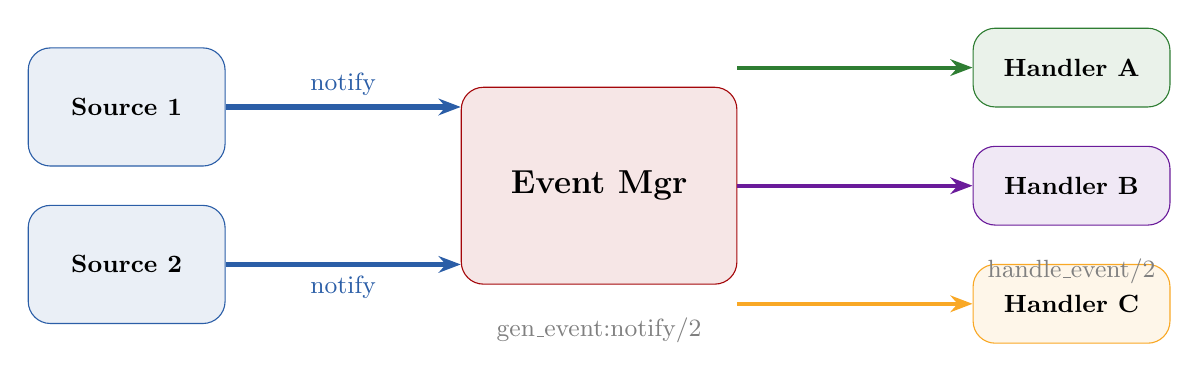
\begin{tikzpicture}
    \node[draw=erlblue, fill=erlblue!10, rounded corners=8pt, minimum width=2.5cm, minimum height=1.5cm, font=\small\bfseries] (src1) at (0,1) {Source 1};
    \node[draw=erlblue, fill=erlblue!10, rounded corners=8pt, minimum width=2.5cm, minimum height=1.5cm, font=\small\bfseries] (src2) at (0,-1) {Source 2};
    \node[draw=erlred, fill=erlred!10, rounded corners=8pt, minimum width=3.5cm, minimum height=2.5cm, font=\large\bfseries] (mgr) at (6,0) {Event Mgr};
    \node[draw=erlgreen, fill=erlgreen!10, rounded corners=8pt, minimum width=2.5cm, minimum height=1cm, font=\small\bfseries] (h1) at (12,1.5) {Handler A};
    \node[draw=erlpurple, fill=erlpurple!10, rounded corners=8pt, minimum width=2.5cm, minimum height=1cm, font=\small\bfseries] (h2) at (12,0) {Handler B};
    \node[draw=erlyellow, fill=erlyellow!10, rounded corners=8pt, minimum width=2.5cm, minimum height=1cm, font=\small\bfseries] (h3) at (12,-1.5) {Handler C};

    \draw[-{Stealth[length=8pt]}, line width=2pt, erlblue]
        (src1.east) -- node[above, font=\small] {notify} (mgr.west |- src1);
    \draw[-{Stealth[length=8pt]}, line width=2pt, erlblue]
        (src2.east) -- node[below, font=\small] {notify} (mgr.west |- src2);
    \draw[-{Stealth[length=8pt]}, line width=1.5pt, erlgreen]
        (mgr.east |- h1) -- (h1.west);
    \draw[-{Stealth[length=8pt]}, line width=1.5pt, erlpurple]
        (mgr.east |- h2) -- (h2.west);
    \draw[-{Stealth[length=8pt]}, line width=1.5pt, erlyellow]
        (mgr.east |- h3) -- (h3.west);

    \node[below=3mm of mgr, font=\small\color{gray}] {gen\_event:notify/2};
    \node[below=3mm of h2, font=\small\color{gray}] {handle\_event/2};
\end{tikzpicture}

\vspace{3cm}

{\large\color{darkgray} 以 event\_logger 为例，从架构到实践}

\vspace{1cm}

{\normalsize\color{gray} Erlang/OTP $\cdot$ Behavior Pattern $\cdot$ Event-Driven Programming}

\vfill
{\small\today}
\end{titlepage}

% ---- Table of Contents ----
\newpage
\tableofcontents
\newpage


% ============================================================
% Section 1: Overview
% ============================================================
\section{概述}

\subsection{什么是 gen\_event？}

\texttt{gen\_event} 是 OTP 框架中的事件处理行为模式（behavior）。它实现了一个\textbf{事件管理器}（Event Manager），可以动态地添加、删除和替换\textbf{事件处理器}（Event Handler）。

与 \texttt{gen\_server} 的一对一模型不同，\texttt{gen\_event} 是一对多的\textbf{发布--订阅}模型：

\begin{tipbox}[核心思想]
\textbf{gen\_event = 一个进程 + 多个处理器}

\begin{itemize}[leftmargin=1.5em]
    \item \textbf{Event Manager}（\texttt{gen\_event.erl}）：一个进程，负责消息循环、Handler 管理
    \item \textbf{Event Handler}（你的回调模块）：多个模块，各自维护独立的 State
    \item 一个事件会被\textbf{所有}已安装的 Handler 处理（广播语义）
\end{itemize}
\end{tipbox}

\subsection{gen\_event 提供的能力}

\begin{table}[H]
\centering
\begin{tabular}{@{}ll@{}}
\toprule
\textbf{能力} & \textbf{说明} \\
\midrule
异步事件 (notify)      & 发送事件后立即返回，所有 Handler 处理 \\
同步事件 (sync\_notify) & 等待所有 Handler 处理完毕后返回 \\
同步调用 (call)         & 向指定 Handler 发送请求并等待回复 \\
动态 Handler 管理       & 运行时添加、删除、替换 Handler \\
Handler 热替换          & \texttt{swap\_handler} 在不丢失状态的情况下替换 \\
监督 Handler            & \texttt{add\_sup\_handler} 关联调用进程，崩溃时通知 \\
多实例支持              & 同一模块可安装多个实例（\texttt{\{Module, Id\}}） \\
\bottomrule
\end{tabular}
\caption{gen\_event 提供的能力}
\end{table}

\subsection{OTP 源码中的工作流}

以下直接对应 \texttt{gen\_event.erl} 源码中的注释：

\begin{tcolorbox}[colback=codebg, colframe=codeborder, arc=2mm, boxrule=0.5pt,
                  title={\textbf{gen\_event.erl --- Work Flow}},
                  fonttitle=\bfseries\ttfamily, width=\textwidth]
\small\ttfamily
\begin{tabular}{@{}lcl@{}}
gen\_event module &  & Callback module \\
\textsf{-{}-{}-{}-{}-{}-{}-{}-{}-{}-{}-{}-{}-{}-{}-{}-{}-} & & \textsf{-{}-{}-{}-{}-{}-{}-{}-{}-{}-{}-{}-{}-{}-{}-} \\
gen\_event:start\_link  & -{}-{}-{}-{}-> & - \\
gen\_event:add\_handler & -{}-{}-{}-{}-> & Module:init/1 \\
gen\_event:notify       & -{}-{}-{}-{}-> & Module:handle\_event/2 \\
gen\_event:call         & -{}-{}-{}-{}-> & Module:handle\_call/2 \\
-                      & -{}-{}-{}-{}-> & Module:handle\_info/2 \\
gen\_event:delete\_handler & -{}-{}-{}-{}-> & Module:terminate/2 \\
gen\_event:swap\_handler   & -{}-{}-{}-{}-> & Module1:terminate/2 \\
                          &               & Module2:init/1 \\
gen\_event:stop         & -{}-{}-{}-{}-> & Module:terminate/2 \\
-                      & -{}-{}-{}-{}-> & Module:code\_change/3 \\
\end{tabular}
\end{tcolorbox}

\subsection{与 gen\_server 的对比}

\begin{table}[H]
\centering
\begin{tabular}{@{}lll@{}}
\toprule
\textbf{特性} & \textbf{gen\_server} & \textbf{gen\_event} \\
\midrule
进程数       & 1 个进程           & 1 个进程 \\
回调模块     & 1 个模块           & N 个模块 \\
状态         & 1 个 State         & N 个 State（每个 Handler 独立） \\
消息模型     & 请求--响应（call/cast） & 发布--订阅（notify） \\
动态性       & 固定回调模块       & 运行时添加/删除/替换 Handler \\
\bottomrule
\end{tabular}
\caption{gen\_server vs gen\_event}
\end{table}


% ============================================================
% Section 2: Architecture Diagrams
% ============================================================
\section{架构图（通过 Pid）}

使用 \texttt{gen\_event:start\_link()} 启动，不注册名字，通过返回的 Pid 来引用 Event Manager。

\begin{figure}[H]
\centering
\includegraphics[width=\textwidth]{images/gen_event_architecture_pid.pdf}
\caption{架构图（方式一）：通过 PID 引用 --- \texttt{start\_link/0}}
\label{fig:arch-pid}
\end{figure}

\subsection{不注册（使用 PID）}

\begin{lstlisting}[style=erlangstyle]
{ok, Pid} = gen_event:start_link().
%% Add handler by PID:
ok = gen_event:add_handler(Pid, my_handler, Args).
%% Notify by PID:
gen_event:notify(Pid, Event).
%% Call by PID:
gen_event:call(Pid, my_handler, Request).
%% Stop by PID:
gen_event:stop(Pid).
\end{lstlisting}

\subsection{实验演示：本地 PID 场景}

在同一个 Erlang 节点上启动匿名 Event Manager，通过返回的 PID 直接操作。

\begin{lstlisting}[style=shellstyle, caption={PID 场景 --- 匿名 Event Manager}]
(apple@ERICKSUN-MC1)1> {ok, Pid} = gen_event:start_link().
{ok,<0.93.0>}
(apple@ERICKSUN-MC1)2> gen_event:add_handler(Pid,
    event_logger, {stdout}).
ok
(apple@ERICKSUN-MC1)3> gen_event:notify(Pid,
    {info, "System started"}).
ok
(apple@ERICKSUN-MC1)4> gen_event:call(Pid,
    event_logger, get_count).
1
(apple@ERICKSUN-MC1)5> gen_event:which_handlers(Pid).
[event_logger]
(apple@ERICKSUN-MC1)6> gen_event:stop(Pid).
ok
\end{lstlisting}

\begin{notebox}[PID 方式的特点]
\begin{itemize}[leftmargin=1.5em]
    \item PID 是进程的直接引用，无需名字注册
    \item 可以启动多个匿名 Event Manager 实例
    \item PID 仅在本地节点有效，跨节点需要额外处理
    \item 必须自行保存 PID，进程死亡后 PID 失效
\end{itemize}
\end{notebox}


\section{架构图（通过名字）}

使用 \texttt{gen\_event:start\_link(EventMgrRef)} 启动，将 Event Manager 注册到名字表，通过名字引用。

\begin{figure}[H]
\centering
\includegraphics[width=\textwidth]{images/gen_event_architecture_named.pdf}
\caption{架构图（方式二）：通过注册名字引用 --- \texttt{start\_link/1}}
\label{fig:arch-named}
\end{figure}

gen\_event 支持多种进程注册方式：

\subsection{本地注册}

\begin{lstlisting}[style=erlangstyle]
gen_event:start_link({local, my_event_mgr}).
%% All operations use the atom name:
gen_event:add_handler(my_event_mgr, my_handler, Args).
gen_event:notify(my_event_mgr, Event).
gen_event:call(my_event_mgr, my_handler, Request).
gen_event:stop(my_event_mgr).
%% Only visible on current node
\end{lstlisting}

\paragraph{实验演示：本地注册在集群中互不影响}

本地注册（\texttt{\{local, Name\}}）的名字仅在当前节点可见。在集群中，\textbf{每个节点可以各自注册同名 Event Manager，互不影响}。

\textbf{节点 apple} --- 启动并注册 \texttt{my\_local\_event\_mgr}：

\begin{lstlisting}[style=shellstyle, caption={apple 节点 --- 本地注册 Event Manager}]
(apple@ERICKSUN-MC1)1> {ok, Pid} = gen_event:start_link(
    {local, my_local_event_mgr}).
{ok,<0.93.0>}
(apple@ERICKSUN-MC1)2> whereis(my_local_event_mgr).
<0.93.0>
(apple@ERICKSUN-MC1)3> gen_event:add_handler(
    my_local_event_mgr, event_logger, {stdout}).
ok
(apple@ERICKSUN-MC1)4> gen_event:notify(
    my_local_event_mgr, {info, "Hello from apple"}).
ok
(apple@ERICKSUN-MC1)5> gen_event:call(
    my_local_event_mgr, event_logger, get_count).
1
\end{lstlisting}

\textbf{节点 pear} --- 连接到 apple 后，\texttt{my\_local\_event\_mgr} 在本节点不可见，可以独立注册同名 Event Manager：

\begin{lstlisting}[style=shellstyle, caption={pear 节点 --- 独立注册同名 Event Manager}]
(pear@ERICKSUN-MC1)1> net_adm:ping('apple@ERICKSUN-MC1').
pong
(pear@ERICKSUN-MC1)2> whereis(my_local_event_mgr).
undefined
(pear@ERICKSUN-MC1)3> {ok, _} = gen_event:start_link(
    {local, my_local_event_mgr}).
{ok,<0.102.0>}
(pear@ERICKSUN-MC1)4> gen_event:add_handler(
    my_local_event_mgr, event_logger, {stdout}).
ok
(pear@ERICKSUN-MC1)5> gen_event:notify(
    my_local_event_mgr, {info, "Hello from pear"}).
ok
(pear@ERICKSUN-MC1)6> rpc:call('apple@ERICKSUN-MC1',
    gen_event, call,
    [my_local_event_mgr, event_logger, get_count]).
1
\end{lstlisting}

\begin{tipbox}[本地注册的关键特性]
\begin{itemize}[leftmargin=1.5em]
    \item \texttt{whereis(my\_local\_event\_mgr)} 在 pear 节点上返回 \texttt{undefined}，说明 apple 节点的本地注册名在 pear 上\textbf{不可见}
    \item pear 节点可以独立注册同名的 Event Manager，两个节点上的 Event Manager \textbf{完全独立}
    \item 通过 \texttt{rpc:call/4} 可以以本地注册名调用远程节点上的 Event Manager
    \item 这正是 \texttt{\{local, Name\}} 的语义：名字的作用域仅限于当前 Erlang 节点
\end{itemize}
\end{tipbox}

\subsection{全局注册}

\begin{lstlisting}[style=erlangstyle]
gen_event:start_link({global, my_global_event_mgr}).
%% All operations use {global, Name}:
gen_event:add_handler({global, my_global_event_mgr},
    my_handler, Args).
gen_event:notify({global, my_global_event_mgr}, Event).
gen_event:call({global, my_global_event_mgr},
    my_handler, Request).
gen_event:stop({global, my_global_event_mgr}).
%% Visible on all connected nodes (distributed)
\end{lstlisting}

\paragraph{实验演示：全局注册在集群中唯一可见}

全局注册（\texttt{\{global, GlobalName\}}）的名字通过 \texttt{global} 模块在整个集群中维护，\textbf{所有连接的节点都能看到并直接使用}。

\textbf{节点 apple} --- 启动并全局注册 \texttt{my\_global\_event\_mgr}：

\begin{lstlisting}[style=shellstyle, caption={apple 节点 --- 全局注册 Event Manager}]
(apple@ERICKSUN-MC1)1> {ok, Pid} = gen_event:start_link(
    {global, my_global_event_mgr}).
{ok,<0.93.0>}
(apple@ERICKSUN-MC1)2> global:registered_names().
[my_global_event_mgr]
(apple@ERICKSUN-MC1)3> gen_event:add_handler(
    {global, my_global_event_mgr}, event_logger, {stdout}).
ok
(apple@ERICKSUN-MC1)4> gen_event:notify(
    {global, my_global_event_mgr},
    {info, "Hello from apple"}).
ok
\end{lstlisting}

\textbf{节点 pear} --- 连接到 apple 后，\texttt{my\_global\_event\_mgr} 在 pear 节点上\textbf{直接可见}：

\begin{lstlisting}[style=shellstyle, caption={pear 节点 --- 直接通过全局名字访问}]
(pear@ERICKSUN-MC1)1> net_adm:ping('apple@ERICKSUN-MC1').
pong
(pear@ERICKSUN-MC1)2> global:registered_names().
[my_global_event_mgr]
(pear@ERICKSUN-MC1)3> gen_event:notify(
    {global, my_global_event_mgr},
    {info, "Hello from pear"}).
ok
(pear@ERICKSUN-MC1)4> gen_event:call(
    {global, my_global_event_mgr},
    event_logger, get_count).
2
\end{lstlisting}

\begin{tipbox}[全局注册的关键特性]
\begin{itemize}[leftmargin=1.5em]
    \item \texttt{global:registered\_names()} 在 pear 节点上也返回 \texttt{[my\_global\_event\_mgr]}，说明全局名字在\textbf{整个集群中可见}
    \item pear 节点无需 \texttt{rpc:call}，直接使用 \texttt{\{global, my\_global\_event\_mgr\}} 即可操作 apple 上的 Event Manager
    \item 全局名字在集群中\textbf{唯一}：如果 pear 节点也尝试 \texttt{start\_link(\{global, my\_global\_event\_mgr\})}，会因为名字已被占用而失败
    \item 这正是 \texttt{\{global, Name\}} 与 \texttt{\{local, Name\}} 的核心区别：全局注册提供集群级别的单例语义
\end{itemize}
\end{tipbox}

\subsection{emgr\_ref() 完整类型}

\begin{table}[H]
\centering
\begin{tabular}{@{}ll@{}}
\toprule
\textbf{类型} & \textbf{说明} \\
\midrule
\texttt{pid()} & 直接 PID 引用 \\
\texttt{atom()} & 本地注册名 \\
\texttt{\{atom(), node()\}} & 远程节点的本地注册名 \\
\texttt{\{global, GlobalName\}} & 全局注册名 \\
\texttt{\{via, RegMod, ViaName\}} & 自定义注册模块 \\
\bottomrule
\end{tabular}
\caption{emgr\_ref() 类型一览}
\end{table}


% ============================================================
% Section 3: Internal Structure
% ============================================================
\section{内部结构}

\subsection{Handler 列表}

Event Manager 内部维护一个 Handler 列表，每个 Handler 包含模块名、ID 和独立的 State：

\begin{lstlisting}[style=erlangstyle]
%% Internal handler record (simplified)
Handlers = [
    {Module_A, Id_A, State_A, Supervised_A},
    {Module_B, Id_B, State_B, Supervised_B},
    {Module_C, Id_C, State_C, Supervised_C}
]
\end{lstlisting}

\subsection{Handler 标识}

Handler 可以用两种方式标识：

\begin{lstlisting}[style=erlangstyle]
%% Method 1: Module name only (one instance per module)
gen_event:add_handler(Mgr, my_handler, Args).

%% Method 2: {Module, Id} tuple (multiple instances)
gen_event:add_handler(Mgr, {my_handler, instance1}, Args).
gen_event:add_handler(Mgr, {my_handler, instance2}, Args).
\end{lstlisting}

\subsection{消息流转}

\begin{figure}[H]
\centering
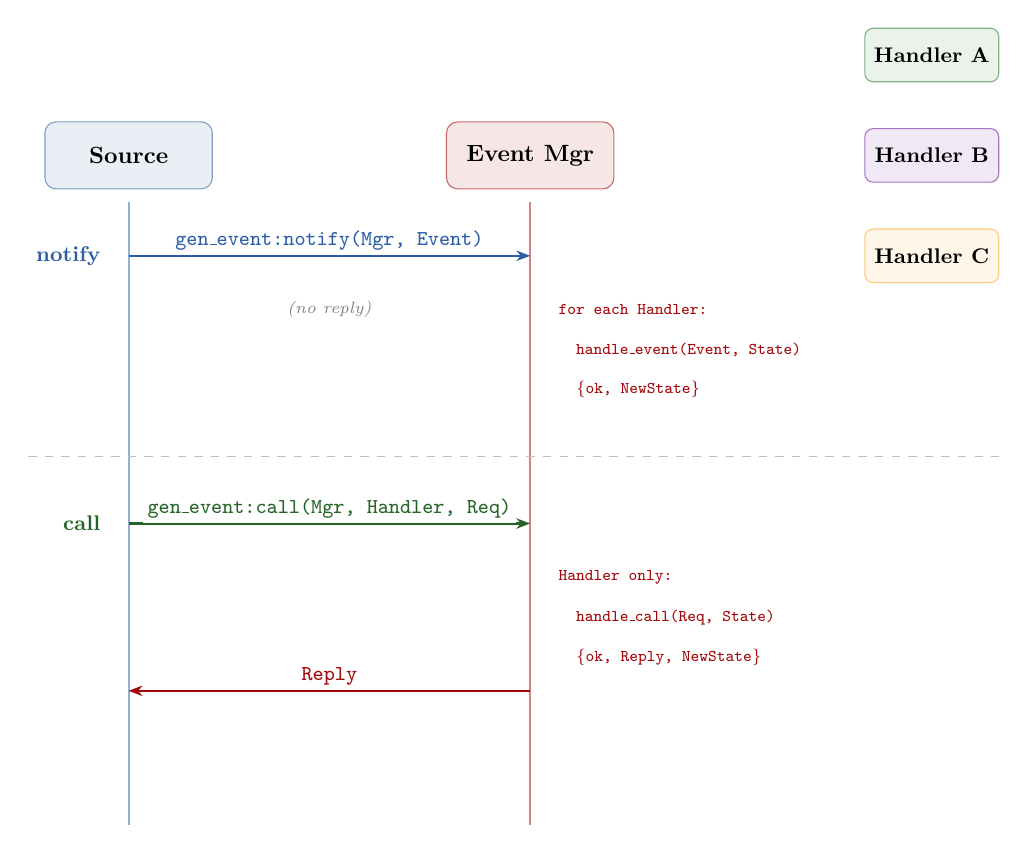
\begin{tikzpicture}[scale=0.85, every node/.style={scale=0.85},
    actor/.style={draw, rounded corners=4pt, fill=#1!10, draw=#1!60,
                  minimum width=2.5cm, minimum height=1cm, font=\bfseries},
    handler/.style={draw, rounded corners=3pt, fill=#1!10, draw=#1!60,
                    minimum width=2cm, minimum height=0.8cm, font=\small\bfseries},
    msg/.style={-{Stealth[length=5pt]}, thick, #1},
    lbl/.style={font=\small\ttfamily, fill=white, inner sep=2pt},
]
    \node[actor=erlblue] (source) at (0, 0) {Source};
    \node[actor=erlred] (mgr) at (6, 0) {Event Mgr};
    \node[handler=erlgreen] (ha) at (12, 1.5) {Handler A};
    \node[handler=erlpurple] (hb) at (12, 0) {Handler B};
    \node[handler=erlyellow] (hc) at (12, -1.5) {Handler C};

    \draw[thick, erlblue!50] (0, -0.7) -- (0, -10);
    \draw[thick, erlred!50] (6, -0.7) -- (6, -10);

    % === notify ===
    \node[font=\small\bfseries\color{erlblue}, anchor=east] at (-0.3, -1.5) {notify};
    \draw[msg=erlblue] (0, -1.5) -- node[lbl, above] {gen\_event:notify(Mgr, Event)} (6, -1.5);
    \node[font=\scriptsize\ttfamily, anchor=west, text=erlred] at (6.3, -2.3) {for each Handler:};
    \node[font=\scriptsize\ttfamily, anchor=west, text=erlred] at (6.3, -2.9) {\ \ handle\_event(Event, State)};
    \node[font=\scriptsize\ttfamily, anchor=west, text=erlred] at (6.3, -3.5) {\ \ \{ok, NewState\}};
    \node[font=\scriptsize\itshape\color{gray}] at (3, -2.3) {(no reply)};

    % === call ===
    \node[font=\small\bfseries\color{erlgreen!80!black}, anchor=east] at (-0.3, -5.5) {call};
    \draw[msg=erlgreen!80!black] (0, -5.5) -- node[lbl, above] {gen\_event:call(Mgr, Handler, Req)} (6, -5.5);
    \node[font=\scriptsize\ttfamily, anchor=west, text=erlred] at (6.3, -6.3) {Handler only:};
    \node[font=\scriptsize\ttfamily, anchor=west, text=erlred] at (6.3, -6.9) {\ \ handle\_call(Req, State)};
    \node[font=\scriptsize\ttfamily, anchor=west, text=erlred] at (6.3, -7.5) {\ \ \{ok, Reply, NewState\}};
    \draw[msg=erlred] (6, -8) -- node[lbl, above] {Reply} (0, -8);

    % Dashed separator
    \draw[dashed, gray!50] (-1.5, -4.5) -- (13, -4.5);
\end{tikzpicture}
\caption{gen\_event 两种消息类型的流转过程}
\label{fig:message-flow}
\end{figure}

\begin{notebox}[notify vs call]
\begin{itemize}[leftmargin=1.5em]
    \item \texttt{notify/2}：异步，\textbf{所有} Handler 都会收到事件
    \item \texttt{sync\_notify/2}：同步，等待所有 Handler 处理完毕
    \item \texttt{call/3,4}：同步，只有\textbf{指定的} Handler 收到请求并返回回复
\end{itemize}
\end{notebox}


% ============================================================
% Section 4: Example — event_logger
% ============================================================
\section{实例：event\_logger}

\begin{notebox}[源码文件]
\texttt{src/event\_logger.erl}
\end{notebox}

以一个事件日志器为例，展示 gen\_event 的核心结构。

\subsection{模块结构}

\begin{itemize}[leftmargin=2em]
    \item \textbf{模块声明}：\texttt{-behaviour(gen\_event).} 声明行为模式
    \item \textbf{init/1}：初始化 Handler State，支持 stdout 和 file 两种输出模式
    \item \textbf{handle\_event/2}：处理 \texttt{notify/sync\_notify} 发来的事件，格式化并输出日志
    \item \textbf{handle\_call/2}：处理 \texttt{gen\_event:call} 发来的同步请求（如查询计数）
    \item \textbf{handle\_info/2}：处理发送到 Event Manager 进程的其他消息
    \item \textbf{terminate/2}：Handler 被删除或 Event Manager 停止时的清理工作
    \item \textbf{code\_change/3}：热代码升级
\end{itemize}

\subsection{使用方式}

\begin{lstlisting}[style=erlangstyle]
%% 1. Start event manager
{ok, Mgr} = gen_event:start_link({local, my_event_mgr}).

%% 2. Add handler
ok = gen_event:add_handler(my_event_mgr, event_logger, {stdout}).

%% 3. Send events (async - all handlers receive)
gen_event:notify(my_event_mgr, {info, "System started"}).
gen_event:notify(my_event_mgr, {error, "Connection lost"}).

%% 4. sync_notify - blocks until all handlers have processed
gen_event:sync_notify(my_event_mgr, {info, "Sync event"}).

%% 5. Query specific handler (sync)
Count = gen_event:call(my_event_mgr, event_logger, get_count).

%% 6. Remove handler
gen_event:delete_handler(my_event_mgr, event_logger, normal).

%% 7. Stop event manager
gen_event:stop(my_event_mgr).
\end{lstlisting}


% ============================================================
% Section 5: Multiple Handlers
% ============================================================
\section{多处理器模式}

\begin{notebox}[源码文件]
\texttt{src/multi\_handler\_demo.erl}
\end{notebox}

\subsection{同一模块的多个实例}

使用 \texttt{\{Module, Id\}} 形式可以安装同一模块的多个实例，每个实例有独立的 State：

\begin{lstlisting}[style=erlangstyle]
%% Add 3 instances of the same handler module
ok = gen_event:add_handler(Mgr, {my_handler, error_filter},
                           #{level => error}).
ok = gen_event:add_handler(Mgr, {my_handler, all_events},
                           #{level => all}).
ok = gen_event:add_handler(Mgr, {my_handler, warning_filter},
                           #{level => warning}).

%% Query specific instance
{ok, Count} = gen_event:call(Mgr,
    {my_handler, error_filter}, get_count).

%% Delete specific instance
gen_event:delete_handler(Mgr,
    {my_handler, error_filter}, normal).
\end{lstlisting}

\begin{warnbox}[Handler ID 必须匹配]
如果 Handler 以 \texttt{\{Module, Id\}} 形式添加，则 \texttt{call}、\texttt{delete\_handler} 等操作也必须使用相同的 \texttt{\{Module, Id\}} 形式，不能只用 \texttt{Module}。
\end{warnbox}


% ============================================================
% Section 6: Swap Handler
% ============================================================
\section{处理器热替换 (swap\_handler)}

\begin{notebox}[源码文件]
\texttt{src/swap\_handler\_demo.erl}
\end{notebox}

\subsection{swap\_handler 机制}

\texttt{swap\_handler} 允许在不丢失状态的情况下替换 Handler：

\begin{enumerate}[leftmargin=2em]
    \item 旧 Handler 的 \texttt{terminate/2} 被调用，返回 \texttt{TransferData}
    \item 新 Handler 的 \texttt{init/1} 接收 \texttt{\{NewArgs, TransferData\}}
    \item 状态在新旧 Handler 之间无缝传递
\end{enumerate}

\begin{lstlisting}[style=erlangstyle]
%% Swap: old handler -> new handler
gen_event:swap_handler(
    Manager,
    {OldHandler, Args1},  %% terminate(Args1, State) -> TransferData
    {NewHandler, Args2}   %% init({Args2, TransferData}) -> {ok, State}
).
\end{lstlisting}

\subsection{实际应用场景}

\begin{itemize}[leftmargin=2em]
    \item 日志输出从文件切换到控制台（保留计数器等状态）
    \item 升级 Handler 版本（保留业务状态）
    \item OTP 的 \texttt{alarm\_handler} 就是通过 swap 来替换默认处理器
\end{itemize}

\begin{lstlisting}[style=erlangstyle]
%% OTP alarm_handler typical usage
gen_event:swap_handler(
    alarm_handler,
    {alarm_handler, swap},        %% Remove default handler
    {my_alarm_handler, MyArgs}    %% Install custom handler
).
\end{lstlisting}


% ============================================================
% Section 7: Supervised Handler
% ============================================================
\section{监督处理器 (add\_sup\_handler)}

\begin{notebox}[源码文件]
\texttt{src/sup\_handler\_demo.erl}
\end{notebox}

\subsection{问题：Handler 崩溃怎么办？}

普通 \texttt{add\_handler} 添加的 Handler 如果崩溃，会被\textbf{静默移除}，没有任何通知。这在生产环境中是不可接受的。

\subsection{add\_sup\_handler 的作用}

\texttt{add\_sup\_handler} 将 Handler 与调用进程关联。当 Handler 被移除（无论是崩溃还是正常删除），调用进程会收到消息：

\begin{lstlisting}[style=erlangstyle]
{gen_event_EXIT, Handler, Reason}
\end{lstlisting}

\subsection{崩溃恢复模式}

\begin{lstlisting}[style=erlangstyle]
watcher_loop(Manager) ->
    receive
        {gen_event_EXIT, my_handler, Reason} ->
            io:format("Handler crashed: ~p~n", [Reason]),
            gen_event:add_sup_handler(Manager, my_handler, []),
            watcher_loop(Manager)
    end.
\end{lstlisting}

\subsection{add\_sup\_handler vs add\_handler}

\begin{table}[H]
\centering
\begin{tabular}{@{}lll@{}}
\toprule
\textbf{特性} & \textbf{add\_handler} & \textbf{add\_sup\_handler} \\
\midrule
Handler 崩溃通知 & 静默移除 & 发送 gen\_event\_EXIT \\
调用进程退出     & Handler 不受影响 & Handler 被移除 \\
适用场景         & 临时/测试 & 生产环境 \\
\bottomrule
\end{tabular}
\caption{add\_handler vs add\_sup\_handler}
\end{table}


% ============================================================
% Section 8: Alarm System
% ============================================================
\section{实战案例：告警系统}

\begin{notebox}[源码文件]
\texttt{src/alarm\_system.erl}
\end{notebox}

一个类似 OTP \texttt{alarm\_handler} 的告警管理系统：

\begin{lstlisting}[style=erlangstyle]
%% Start the alarm manager
alarm_system:start_link().

%% Set an alarm
alarm_system:set_alarm(cpu_high, "CPU usage above 90%").

%% Clear an alarm
alarm_system:clear_alarm(cpu_high).

%% Get all active alarms
{ok, Alarms} = alarm_system:get_alarms().
\end{lstlisting}

告警系统展示了 gen\_event 在实际生产中的典型用法：
\begin{itemize}[leftmargin=2em]
    \item Event Manager 作为告警总线
    \item Handler 维护活跃告警列表
    \item 支持设置、清除、查询告警
    \item 重复设置同一告警会更新而非重复
\end{itemize}


% ============================================================
% Section 9: Callback Return Values
% ============================================================
\section{回调函数返回值}

\subsection{init/1}

\begin{lstlisting}[style=erlangstyle]
init(Args) ->
    {ok, State}              %% Normal initialization
  | {ok, State, hibernate}   %% Init and hibernate
  | {error, Reason}.         %% Initialization failed
\end{lstlisting}

\begin{warnbox}[注意]
与 gen\_server 不同，\texttt{init} 失败\textbf{不会}导致 Event Manager 崩溃，只是该 Handler 不会被安装。
\end{warnbox}

\subsection{handle\_event/2}

\begin{lstlisting}[style=erlangstyle]
handle_event(Event, State) ->
    {ok, NewState}                %% Continue
  | {ok, NewState, hibernate}     %% Continue, hibernate
  | {swap_handler, Args1, NewState, Handler2, Args2}
  | remove_handler.               %% Remove this handler
\end{lstlisting}

\subsection{handle\_call/2}

\begin{lstlisting}[style=erlangstyle]
handle_call(Request, State) ->
    {ok, Reply, NewState}              %% Reply and continue
  | {ok, Reply, NewState, hibernate}   %% Reply, hibernate
  | {swap_handler, Reply, Args1, NewState, Handler2, Args2}
  | {remove_handler, Reply}.           %% Reply and remove
\end{lstlisting}

\subsection{handle\_info/2}

返回值与 \texttt{handle\_event/2} 相同。

\subsection{terminate/2}

\begin{lstlisting}[style=erlangstyle]
terminate(Reason, State) ->
    term().  %% Return value used as TransferData in swap
\end{lstlisting}

\textbf{Reason 的值}：
\begin{itemize}[leftmargin=2em]
    \item \texttt{stop} --- Event Manager 正在停止
    \item \texttt{\{stop, Reason\}} --- Event Manager 被要求停止
    \item \texttt{normal} / 自定义 --- \texttt{delete\_handler} 传入的 Args
    \item \texttt{\{error, Term\}} --- Handler 回调返回了错误值
    \item \texttt{\{error, \{'EXIT', Reason\}\}} --- Handler 回调崩溃
\end{itemize}

\begin{warnbox}[重要]
当用于 \texttt{swap\_handler} 时，\texttt{terminate} 的返回值会传递给新 Handler 的 \texttt{init}。
\end{warnbox}


% ============================================================
% Section 10: Best Practices
% ============================================================
\section{最佳实践与常见陷阱}

\subsection{最佳实践}

\begin{enumerate}[leftmargin=2em]
    \item \textbf{使用 add\_sup\_handler}：生产环境中始终使用监督处理器
    \item \textbf{Handler 保持轻量}：避免在 \texttt{handle\_event} 中做耗时操作
    \item \textbf{处理未知事件}：总是添加 catch-all 子句
    \item \textbf{利用 swap\_handler}：需要升级 Handler 时使用，而非 delete + add
    \item \textbf{notify vs sync\_notify}：
    \begin{itemize}[leftmargin=1.5em]
        \item \texttt{notify}：fire-and-forget，高吞吐
        \item \texttt{sync\_notify}：需要确保事件被处理完毕时使用
    \end{itemize}
\end{enumerate}

\subsection{常见陷阱}

\subsubsection{陷阱 1：Handler 崩溃被静默吞掉}

\begin{lstlisting}[style=erlangstyle]
%% BAD: handler crashes silently
gen_event:add_handler(Mgr, my_handler, []).

%% GOOD: get notified on crash
gen_event:add_sup_handler(Mgr, my_handler, []).
\end{lstlisting}

\subsubsection{陷阱 2：阻塞其他 Handler}

\begin{lstlisting}[style=erlangstyle]
%% BAD: blocks all other handlers
handle_event(Event, State) ->
    timer:sleep(5000),  %% All handlers are blocked!
    {ok, State}.

%% GOOD: spawn for heavy work
handle_event(Event, State) ->
    spawn(fun() -> heavy_processing(Event) end),
    {ok, State}.
\end{lstlisting}

\subsubsection{陷阱 3：忘记 swap\_handler 的 terminate 返回值}

\begin{lstlisting}[style=erlangstyle]
%% terminate must return transfer data when swapping
terminate({swap_to, _}, State) ->
    State;  %% This becomes TransferData for new handler
terminate(_Reason, _State) ->
    ok.     %% Normal termination
\end{lstlisting}

\subsubsection{陷阱 4：call 错误的 Handler ID}

\begin{lstlisting}[style=erlangstyle]
%% If handler was added as {Module, Id}:
gen_event:add_handler(Mgr, {my_mod, inst1}, []).

%% Must use same form to call:
gen_event:call(Mgr, {my_mod, inst1}, request).  %% Correct
gen_event:call(Mgr, my_mod, request).           %% WRONG!
\end{lstlisting}


% ============================================================
% Section 11: Quick Reference
% ============================================================
\section{快速参考}

\subsection{Event Manager 函数}

\begin{table}[H]
\centering
\begin{tabular}{@{}ll@{}}
\toprule
\textbf{函数} & \textbf{说明} \\
\midrule
\texttt{gen\_event:start\_link(\{local,N\})} & 启动并本地注册 \\
\texttt{gen\_event:start\_link(\{global,N\})} & 启动并全局注册 \\
\texttt{gen\_event:start\_link()} & 启动不注册 \\
\texttt{gen\_event:start(...)} & 同上但不链接 \\
\texttt{gen\_event:stop(Ref)} & 停止 Event Manager \\
\bottomrule
\end{tabular}
\caption{Event Manager 函数}
\end{table}

\subsection{Handler 管理函数}

\begin{table}[H]
\centering
\begin{tabular}{@{}ll@{}}
\toprule
\textbf{函数} & \textbf{说明} \\
\midrule
\texttt{add\_handler(Mgr, Handler, Args)} & 添加 Handler \\
\texttt{add\_sup\_handler(Mgr, Handler, Args)} & 添加监督 Handler \\
\texttt{delete\_handler(Mgr, Handler, Args)} & 删除 Handler \\
\texttt{swap\_handler(Mgr, \{H1,A1\}, \{H2,A2\})} & 替换 Handler \\
\texttt{swap\_sup\_handler(Mgr, \{H1,A1\}, \{H2,A2\})} & 替换为监督 Handler \\
\texttt{which\_handlers(Mgr)} & 列出所有 Handler \\
\bottomrule
\end{tabular}
\caption{Handler 管理函数}
\end{table}

\subsection{事件发送函数}

\begin{table}[H]
\centering
\begin{tabular}{@{}lll@{}}
\toprule
\textbf{函数} & \textbf{类型} & \textbf{说明} \\
\midrule
\texttt{notify(Mgr, Event)} & 异步 & 发送事件，立即返回 \\
\texttt{sync\_notify(Mgr, Event)} & 同步 & 等待所有 Handler 处理完 \\
\texttt{call(Mgr, Handler, Req)} & 同步 & 向指定 Handler 发请求 \\
\texttt{call(Mgr, Handler, Req, Timeout)} & 同步 & 带超时 \\
\bottomrule
\end{tabular}
\caption{事件发送函数}
\end{table}

\subsection{源码文件列表}

\begin{table}[H]
\centering
\begin{tabular}{@{}ll@{}}
\toprule
\textbf{文件} & \textbf{说明} \\
\midrule
\texttt{src/event\_logger.erl} & 基本用法：事件日志器 \\
\texttt{src/event\_counter.erl} & ETS 事件计数器 \\
\texttt{src/multi\_handler\_demo.erl} & 多处理器（同模块多实例） \\
\texttt{src/swap\_handler\_demo.erl} & 处理器热替换 \\
\texttt{src/alarm\_system.erl} & 实战：告警管理系统 \\
\texttt{src/sup\_handler\_demo.erl} & 监督处理器与崩溃恢复 \\
\texttt{src/counter\_event\_pid.erl} & emgr\_ref 演示：PID 方式 \\
\texttt{src/counter\_event\_local.erl} & emgr\_ref 演示：本地注册 \\
\texttt{src/counter\_event\_global.erl} & emgr\_ref 演示：全局注册 \\
\bottomrule
\end{tabular}
\caption{源码文件列表}
\end{table}

\subsection{Makefile 命令}

\begin{lstlisting}[style=shellstyle, caption={src/Makefile 可用命令}]
make compile     # Compile all .erl files
make run_logger  # Event logger demo (basic usage)
make run_counter # Event counter demo (ETS + handle_call)
make run_multi   # Multiple handlers demo
make run_swap    # Swap handler demo (hot-swap)
make run_alarm   # Alarm system demo (practical example)
make run_sup     # Supervised handler demo (add_sup_handler)
make run_local   # emgr_ref demo: local name
make run_global  # emgr_ref demo: global name
make run_pid     # emgr_ref demo: pid (anonymous)
make run_all     # Run all demos sequentially
make clean       # Remove compiled files
\end{lstlisting}


\end{document}
